% !Mode:: "TeX:UTF-8"
%% 请使用 XeLaTeX 编译本文.
% \documentclass{YAUthesis}% 选项 forprint: 交付打印时添加, 避免彩色链接字迹打印偏淡. 即使用下一行:
% !TEX program = xelatex
 \documentclass[forprint]{YAUthesis}

\begin{document}
%%%%%%% 下面的内容, 据实填空.


\miji{一般}                    % 密级. 没有就空着.
\StudentNumber{1060315024011} % 填写自己的学号
\ClassNumber{TPXXX.xx}				%分类号
\DepartNumber{06}				%单位代码, 参考学校发的文件
\title{本科毕业论文(设计)}
\Titleo{How to use YAUthesis} %题目1 第一行题目
\Titlet{Happy ~\LaTeX~ing}		%题目2 第二行题目(一行不够的情况下填写) 需要取去掉YAUthesis.cls中 82 83行前面的%
\author{赵驰}                            % 作者名字
\Csupervisor{马乐荣}        %指导教师中文名
\PRAT{副教授} 							%指导教师职称professional ranks and titles
\Cmajor{计算机科学与技术}                  % 专业中文名
\Cschoolname{计算机科学与技术学院}          % 学院名
\date{二零一九年五月}                    % 日期
\abstractCn{中文摘要} %中文摘要
\abstractEn{abstractEn} %英文摘要

%-----------------------------------------------------------------------------
\pdfbookmark[0]{封面}{title}         % 封面页加到 pdf 书签
\maketitle
\frontmatter
\pagenumbering{Roman}              % 正文之前的页码用大写罗马字母编号.
%-----------------------------------------------------------------------------
% !Mode:: "TeX:UTF-8"

%%% 此部分需要自行填写: (1) 中文摘要及关键词 (2) 英文摘要及关键词
%%%%%%%%%%%%%%%%%%%%%%%%%%%%%

%%% 郑重声明部分无需改动
%%%---- 郑重声明 (无需改动)------------------------------------%
\newpage
\vspace*{20pt}
\begin{center}
	{\heiti\zihao{3}延安大学学士学位论文原创性声明}
\end{center}
\par\vspace*{10pt}
\renewcommand{\baselinestretch}{1.5}

{\zihao{4}%

本人郑重声明:所呈交的学位论文,是本人在指导教师的指导下,独立进行研究所取得的成果。除文中已经注明引用的内容外,本论文不含任何其他个人或集体已经发表或撰写过的作品成果。对本文的研究做出重要贡献的个人和集体,均已在文中以明确方式标明。本人完全意识到本声明的法律结果由本人承担。\\[5mm]

\hspace*{1cm}本人签名: $\underline{\hspace{3.5cm}}$
\hspace{2cm}日期: $\underline{\hspace{3.5cm}}$\hfill\par}
\vskip20mm

\begin{center}
	{\heiti\zihao{3}关于论文使用授权的说明}
\end{center}
\par\vspace*{10pt}

{\zihao{3}%
	
学位论文作者完全了解延安大学有关保留和使用论文的规定,即:本科生在校攻读学士学位期间论文工作的知识产权单位属延安大学,学生公开发表需经指导教师同意。学校有权保留并向国家有关部门或机构送交论文的复印件,允许学位论文被查阅和借阅;学校可以公布学位论文的全部或部分内容,可以允许采用影印、缩印或其它复制手段保存、汇编学位论文。

论文注释:本学位论文不属于保密范围,适用本授权书。\\[5mm]
	
	\hspace*{1cm}本人签名: $\underline{\hspace{3.5cm}}$
	\hspace{2cm}日期: $\underline{\hspace{3.5cm}}$\hfill\par 
	\vskip5mm
	\hspace*{1cm}导师签名: $\underline{\hspace{3.5cm}}$
	\hspace{2cm}日期: $\underline{\hspace{3.5cm}}$\hfill\par}
%------------------------------------------------------------------------------
\baselineskip=18pt  % 正文行距为 18 磅
%------------------------------------------------------------------------------





%%======中文摘要===========================%
\begin{cnabstract}
本文主要介绍和讨论了延安大学本科毕业论文的~\LaTeX~模板.
指明了编译方法, 也指出了一些常见的排版错误. 

本文的创新点主要有:
\begin{itemize}
	\item 引入~mhchem~和~chemfig~, 支持有机化学式排版; 
	\item 引入~listings~和~algorithm2e~, 支持代码与伪代码排版; 
	\item 引入~booktabs~, 可以控制表线粗细;
\end{itemize}

使用本模板的过程中,如有任何关于本模板的疑问或是不懂之处可通过以下方式联系作者:

\begin{itemize}
	\item 邮箱:dandanv5@hotmail.com
\end{itemize}

\end{cnabstract}
\par
\vspace*{2em}


%%%%--  关键词 -----------------------------------------%%%%%%%%
%%%%-- 注意: 每个关键词之间用“;”分开,最后一个关键词不打标点符号
\cnkeywords{毕业论文; \LaTeX{}; 模板  }


%%====英文摘要==========================%


\begin{enabstract}
This thesis is a study on the theory of \dots.

\end{enabstract}
\par
\vspace*{2em}

%%%%%-- Key words --------------------------------------%%%%%%%
%%%%-- 注意: 每个关键词之间用“;”分开,最后一个关键词不打标点符号
 \enkeywords{\LaTeX{}}
    % 加入摘要, 申明.
%==========================把目录加入到书签==============================%%%%%%
\pdfbookmark[0]{目录}{toc}
\tableofcontents
\mainmatter %% 以下是正文
%%%%%%%%%%%%%%%%%%%%%%%%%%%--------main matter-------%%%%%%%%%%%%%%%%%%%%%%%%%%%%%%%%%%%%
\chapter{引言}

\section{模板结构}

模板文件的结构, 如下表所示:
 \begin{table}[ht]\centering
\begin{tabular}{r|r|l}
	\hline\hline
	\multicolumn{2}{l|}{YAUthesis.tex }       & 主文档. 在其中填写正文.             \\ \hline
	                                & frontmatter.tex & 郑重声明、中英文摘要.               \\ \cline{2-3}
	\raisebox{1em}{includefile 文件夹} &  backmatter.tex & 致谢.                       \\ \hline
	\multicolumn{2}{l|}{figures 文件夹}                  & 存放图片文件.                   \\ \hline
	\multicolumn{2}{l|}{YAUthesis.cls }             & 定义文档格式的 class file. 不可删除. \\ \hline\hline
\end{tabular}
\end{table}

无需也不要改变、移动上述文档的位置.


利用~TexStudio~或者~VScode~, 可以更方便地管理这些文件:
\begin{itemize}
    \item TexStudio: 解压该压缩包, 直接打开~tex~文件;
    \item VScode: 解压该压缩包, 按住~shift~在程序根目录中选择~open with VScode~;
\end{itemize} 

 \section{使用步骤}

 \begin{description}

  \item[Step 1]  进入 includefile 文件夹,  打开 frontmatter.tex, backmatter.tex 这两个文档,
        分别填写 (1) 中文摘要、英文摘要, (2) 致谢.

  \item[Step 2]  打开主文档 YAUthesis.tex, 填写题目、作者等等信息, 书写正文. 如果论文标题太长, 请打开~YAUthesis.cls~这个文档, 去掉第80和81行最前面的\%.

  \item[Step 3]  使用 XeLaTeX 编译. 具体见 \ref{sec-compile} 节.


\end{description}


\section{编译方法} \label{sec-compile}

默认使用 XeLaTeX 编译, 直接生成~pdf 文件.

Windows用户使用TexStudio+Texlive2018或VScode+Texlive2018, 配置方法见我博客: \url{https://blog.i-ll.cc/archives/501
}.   




\section{文档类型选择}
文档类型有 2 种情形:

\begin{table}[ht]\centering
\begin{tabular}{ll}
\hline
   \verb|\documentclass{YAUthesis}|                     &  毕业论文 \\
   \verb|\documentclass[forprint]{YAUthesis}|        &  毕业论文打印版 \\
\hline
\end{tabular}
\end{table}
相关解释见下节.


\section{打印的问题}
\begin{enumerate}[i)]
%  \item  论文要求\colorbox{yellow}{单面打印}.
  \item  关于文档选项 forprint: 交付打印时, 建议加上选项 forprint, 以消除链接文字之彩色, 避免打印字迹偏淡.
  \item  打印时留意不要缩小页面或居中. 即页面放缩方式应该是``无''(Adobe Reader XI 是选择``实际大小'').
           有可能页面放缩方式默认为``适合可打印区域'', 会导致打印为原页面大小的 $97\%$.
           文字不要居中打印, 是因为考虑到装订, 左侧的空白留得稍多一点(模板已作预留).
\end{enumerate}
%如果不是彩色打印机, 请在打印时, 选择将彩色打印为黑白, 否则彩色文字打出的墨迹会偏淡.

\textbf{问}: {\kaishu 生成 PDF 文件时, 不能去掉目录和文章的引用彩色方框, 请问怎么解决?}

\textbf{答}: {\kaishu 方框表示超级链接, 只在电脑上看得见. 实际打印时, 是没有的. 另外, 文档类型加选项 forprint 之后, 这些框框会隐掉的. }

 \vfill

本文档下载更新地址: \url{https://github.com/MLZC/YAUthesis/releases}. 使用之前, 请移步查看是否有更新.

问题反馈及建议, 请联系: dandanv5@hotmail.com.



\chapter{其他操作}


 \section{字体调节}

\begin{tabular}{ll}
	\verb|\songti|   & {\songti 宋体}   \\
	\verb|\bfseries|    & {\bfseries 粗宋体}    \\
	\verb|\sffamily| & {\sffamily 黑体} \\
	\verb|\bfseries\sffamily| & {\bfseries\sffamily 粗黑体} \\
  \verb|\ttfamily|   & {\ttfamily 仿宋}   \\
  \verb|\bfseries\ttfamily|   & {\bfseries\ttfamily 粗仿宋}   \\
  \verb|\itshape|   & {\itshape 楷书}   \\
  \verb|\bfseries\itshape|   & {\bfseries\itshape 粗楷书}   \\

\end{tabular}
\textbf{}

\section{字号调节}
字号命令: \verb|\zihao| \index{zihao}

\begin{tabular}{ll}
\verb|\zihao{0}| &\zihao{0}  初号字 English \\
\verb|\zihao{-0}|&\zihao{-0} 小初号 English \\
\verb|\zihao{1} |&\zihao{1}  一号字 English \\
\verb|\zihao{-1}|&\zihao{-1} 小一号 English \\
\verb|\zihao{2} |&\zihao{2}  二号字 English \\
\verb|\zihao{-2}|&\zihao{-2} 小二号 English \\
\verb|\zihao{3} |&\zihao{3}  三号字 English \\
\verb|\zihao{-3}|&\zihao{-3} 小三号 English \\
\verb|\zihao{4} |&\zihao{4}  四号字 English \\
\verb|\zihao{-4}|&\zihao{-4} 小四号 English \\
\verb|\zihao{5} |&\zihao{5}  五号字 English \\
\verb|\zihao{-5}|&\zihao{-5} 小五号 English \\
\verb|\zihao{6} |&\zihao{6}  六号字 English \\
\verb|\zihao{-6}|&\zihao{-6} 小六号 English \\
\verb|\zihao{7} |&\zihao{7}  七号字 English \\
\verb|\zihao{8} |&\zihao{8}  八号字 English \\
\end{tabular}

\section{列表的使用}

列表是常用的文本格式. 分别是编号的enumerate环境、不编号的itemize环境和使用关键字的description环境.
另外要说明的是,itemize, enumerate, description 这三种 list 环境, 已经调节了其间距和缩进,
以符合中文书写的习惯.
enumerate环境使用数字自动编号: 

\begin{enumerate}
  \item 中文
  \item English
  \item Français
\end{enumerate}

itemize环境不编号,但是会在每个条目前面加一个符号以示标记: 

\begin{itemize}
  \item 中文
  \item English
  \item Français
\end{itemize}

description环境总是使用\verb|\item |命令的可选参数, 把它作为条目的关键字加粗显示:
参见上一章的栗子.

特殊编号比如:~\verb|\begin{enumerate}[(a)]| 得到形如 (a), (b), (c) 的编号.

\verb|\begin{enumerate}[i)]| 得到形如 i), ii), iii) 的编号.

\verb|\begin{enumerate}1)]| 得到形如 1), 2), 3) 的编号. 栗子如下: 

\begin{enumerate}[1)]
  \item 中文
  \item English
  \item Français
\end{enumerate}


列表环境可以嵌套使用(最多四层),举个栗子: 

\begin{enumerate}
  \item 中文
  \begin{enumerate}
    \item 古代汉语
    \item 现代汉语
    \begin{enumerate}
      \item 口语
      \begin{enumerate}
        \item 普通话
        \item 方言
      \end{enumerate}
      \item 书面语
    \end{enumerate}
  \end{enumerate}
  \item English
  \item Français
\end{enumerate}

\section{标点符号的问题}

建议使用半角的标点符号, 后边再键入一个空格. 特别是在英文书写中要注意此问题!

双引号是由两个左单引号、两个右单引号构成的: \verb|``  ''|. 左单引号在键盘上数字~1 的左边.

但是, 无论您偏向于全角或半角, 强烈建议您使用实心的句号, 只要您书写的是自然科学的文章.
原因可能是因为, 比如使用全角句号的句子结尾处的``$x$. ''容易误为数学式~$x_0$(\verb|$x_0$|)吧.



\section{参考文献的引用}



参考文献的引用, 用命令~\verb|\cite{ }|. 大括号内要填入的字串, 是自命名的文献条目名.

比如, 通常我们会说:

 {\kaishu
关于此问题, 请参见文献 \cite{r2}. 作者某某还提到了某某概念\upcite{r1}.}


上文使用的源文件为:

 {\kaishu
关于此问题, 请参见文献~\verb|\cite{r2}|. 作者某某还提到了某某概念~\verb|\upcite{r1}|.
}

其中~\verb|\upcite| 是自定义命令, 使文献引用呈现为\CJKunderdot{上标形式}.

({\heiti 注意:} {\kaishu 这里文献的引用, 有时需要以上标形式出现, 有时需要作为正文文字出现, 为什么?})

另外, 要得到形如~\cite{r1,r3,r4,r5} 的参考文献连续引用, 需要用到 cite 宏包(模板已经加入),
在正文中使用~\verb|\cite{r1,r3,r4,r5}| 的引用形式即可.
或者, 连续引用的上标形式: 使用~\verb|\upcite{r1,r2,r3}|, 得到\upcite{r1,r2,r3}.


\section{玩转数学公式}

\subsection{定理和公式的引用}

\begin{theorem}[谁发现的]\label{th-abcd}
最大的正整数是~$1$.
\end{theorem}

\begin{proof}
要找到这个最大的正整数, 我们设最大的正整数为~$x$, 则~$x \geqslant 1$, 两边同时乘以~$x$, 得到
\begin{equation}\label{eq-abc}
x^2 \geqslant x.
\end{equation}
而~$x$ 是最大的正整数, 由~\eqref{eq-abc} 式得到
\[
x^2 = x.
\]
所以
\begin{equation*}
x = 1.
\end{equation*}
\end{proof}

定理~\ref{th-abcd} 是一个重大的发现.

\subsection{定义, 推论等环境的使用}
%%%%----- 定义等环境的举例 --------
\begin{definition}[整数]
 正整数(例如 1, 2, 3)、负整数(例如 ${−1}$, $−2$, $−3$)与零(0)合起来统称为{\heiti 整数}.
\end{definition}

\begin{remark}
  整数集合在数学上通常表示为 $\mathbf{Z}$ 或 $\mathbb{Z}$, 该记号源于德语单词 Zahlen(意为``数'')的首字母.
\end{remark}

\begin{proposition}
任意两个整数相加、相减、相乘的结果, 仍然是整数.
\end{proposition}

\begin{example}
  $1+2=3$.
\end{example}

\begin{corollary}
   在整数集合内, 相加、相减、相乘运算是封闭的.
\end{corollary}

\subsection{行内公式, 矩阵, 多行公式栗子}
%%%----行内公式, 矩阵, 多行公式举栗子--%%%
在文中引用公式可以这么写:$a^2+b^2=c^2$这是勾股定理, 它还可以表示为$c=\sqrt{a^2+b^2}$, 还可以让公式单独一段并且加上编号
\begin{equation}\label{eq-pingfanghe}
\sin^2{\theta}+\cos^2{\theta}=1 
\end{equation}
还可以通过添加标签在正文中引用公式, 如式~\eqref{eq-pingfanghe}~
我们还可以轻松打出一个矩阵
\begin{equation}
\bm{A}=\begin{bmatrix} %\bm为数学粗体 \hm为更粗的加重体数学负号
1&2&3&4\\
11&22&33&44\\
\end{bmatrix}
\times\begin{bmatrix}
22&24\\
32&34\\
42&44\\
52&54\\
\end{bmatrix}
\end{equation}

或者多个带编号的公式

\begin{gather}
f_1(x)=12x^2+36x+\sin x\\
f_2(x)=\sqrt{3}{x^3+3x}
\end{gather}

以上

\subsection{化学方程式的使用} 

化学方程式可以直接采用数学式输入, 例如: 
三硝基甲苯(TNT)~C$_6$H$_2$CH$_3$(NO$_2$)$_3$
为白色或苋色淡黄色针状结晶, 无臭, 有吸湿性. 
本品为比较安全的炸药, 能耐受撞击和摩擦, 但任何量突然受热都能引起爆炸. 中等毒性. 

很明显, 将化学方程式作为数学公式输入很复杂, 且十分笨拙. 所以我引入了mhchem宏包
将问题简化. ~\verb|\ce|~命令用来输入化学方程式. 如: 醋中主要是 \ce{H2O}, 含有
 \ce{CH3C00-}. \ce{^{277}_{90}Th}元素具有强放射性.

 化学反应式栗子如下:

 \begin{gather} 
   \ce{2H2 + O2 ->[\text{燃烧}] 2H2O} \\
   \ce{N2 + 3H2 <=>T[高温、加压][催化剂] 2NH3}
 \end{gather}

有机化学式的书写, 先简单介绍一下~chemfig~方向的定义, 如图~\ref{fig:direction}: 

\begin{figure}[ht]
  \centering
    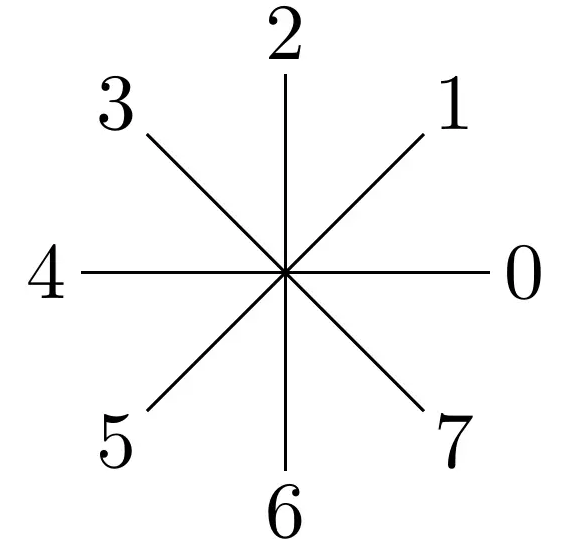
\includegraphics[width=\imagewidth]{direction.png}
    \caption{chemfig方向的定义}
    \label{fig:direction}
\end{figure}

举个乙烷的栗子:

\begin{center}
  \chemfig{C(-[2]H)(-[4]H)(-[6]H)-C(-[2]H)(-[6]H)-H}
\end{center}

上述乙烷代码如下: 

{\verb|\chemfig{C(-[2]H)(-[4]H)(-[6]H)-C(-[2]H)(-[6]H)-H}|}

代码中 (-[X]Y) 内的数字 X 就表示了内容 Y 的位置,
其中中括号([ ])的位置通常紧跟在化学键(-、= 等)之后。

例如 2 表示的就是向上的方向,4 表示向左,6 表示向右。

最后再画一个苯环结束:

\begin{center}
  \chemfig{*6(-=-=-=)}
\end{center}


\section{图的使用}

支持EPS、PDF、PNG、JPEG、BMP格式的图片,
当然也可以用绘图包直接在\LaTeX 中绘制图形, 推荐使用宏包tikz(本模板暂时未加). 

\subsection{单图排版}

用形如~\verb|
\includegraphics[width=12cm]{texlion.jpg}| 的命令可以纳入图片.

如图~\ref{fig:lion} 是一个插入入~jpg 图片的例子.

\begin{figure}[ht]
\centering
  
\includegraphics[width=\imagewidth]{texlion.jpg}
  \caption{一个彩色 jpg 图片的例子}
  \label{fig:lion}
\end{figure}


\subsection{双图排版}

双图排版很简单!


\begin{figure}[ht]
\centering
\begin{minipage}[t]{\imagewidth}
\centering
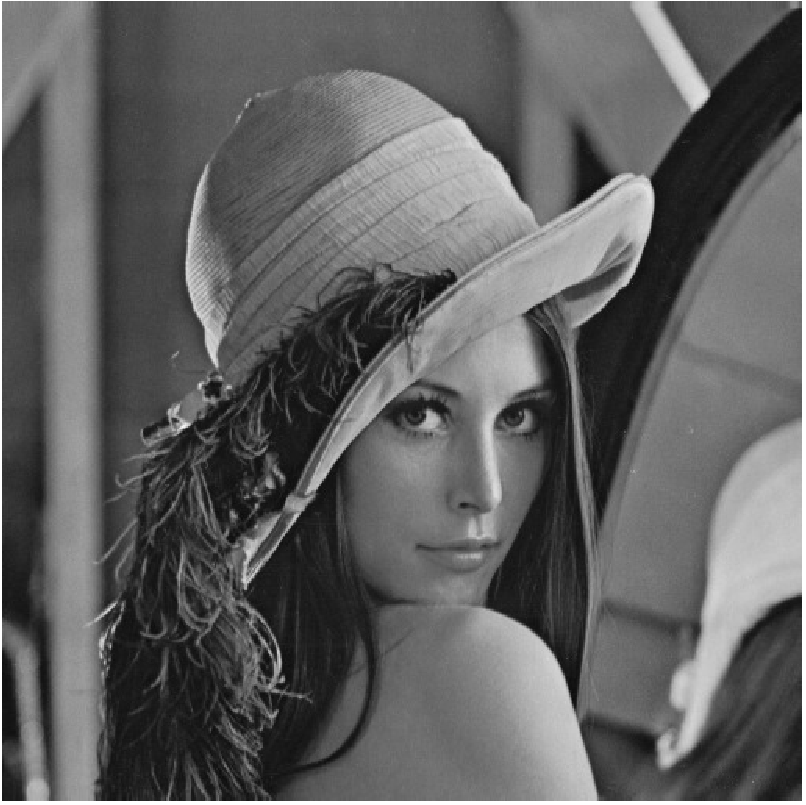
\includegraphics[width=\imagewidth]{Lenna}
a)
\end{minipage} \hspace{4pt}
\begin{minipage}[t]{\imagewidth}
\centering

\includegraphics[width=\imagewidth]{Lenna_e}
b)
\end{minipage}
\caption{A pair of plain-image and the corresponding cipher-image:
a) image ``Lenna''; b) cipher-image of a).}
\label{fig:APairPlaintext}
\end{figure}



\section{表的使用}

作为论文, 推荐使用``三线表'', 如表 \ref{tab:1}. 进行排版. 所谓三线表, 
即在标题前有横线, 标题后有横线, 表格最后还有横线, 其他地方无线. 当然这不是死规定, 
也可以根据需要在合适的地方加线. 



\begin{table}[ht]
\centering
\caption{某校学生身高体重样本}
\label{tab:1}
    \begin{tabular}{ccccc}
    \toprule
    序号&性别&年龄&身高/cm&体重/kg\\
    \midrule
    1&F&14&156&42\\
    2&F&16&158&45\\
    3&M&14&162&48\\
    4&M&15&163&50\\
    \cmidrule{3-5} %添加2-4列的中线
    平均& &15&159.75&46.25\\
    \bottomrule
    \end{tabular}
\end{table}

\section{代码排版}

\subsection{伪代码排版}

伪代码排版使用了algorithm2e,我们来看看算法\ref{qsort}(更多样例请google``algorithm2e''):

\begin{algorithm}[H]\label{qsort}
    \SetAlgoLined
    \KwData{this text}
    \KwResult{how to write algorithm with \LaTeX2e }
    initialization\;
    \While{not at end of this document}{
        read current\;
        \eIf{understand}{
            go to next section\;
            current section becomes this one\;
        }{
            go back to the beginning of current section\;
        }
    }
    \caption{How to write algorithms}
\end{algorithm}

\subsection{代码排版}

Python AI引擎核心代码, 以下代码估值百亿! 
\begin{lstlisting}[language=python, caption={一段估值百亿的AI核心代码ai.py}, label=ai]
  while True:
  print(input("").replace("吗","").replace("?","!"))
\end{lstlisting}

%%%%============================================================================================================%%%

\chapter{更新记录}
2019 年 05 月更新: 更新封面字体格式, 大小, 完善正文中的字体切换命令; 更新标题格式为黑体加粗; 

2019 年 02 月更新: 更新封面以适配延安大学论文要求; 更新标题格式; 更新目录格式; 
适应TexLive2018版本; 删除英文封面;添加booktabs宏包优化表格; 优化图片排版; 
添加化学宏包mhchem, chemfig以及基本栗子; 
添加多行公式、矩阵、行内公式栗子; 添加嵌套列表栗子; 
引入最新伪代码宏包algorithm2e, 代码宏包listings以及基本栗子;
[数计学院2015级赵驰同学]

2016 年 06 月更新: 正文字体为小四号; 英文字体为 Times New Roman; 修订图表标题的字体、字号; 修订目录的字号; 修订附录章节编号的问题. 
                          非常感谢武汉大学数学与统计学院 2012 级张仕俊、林颖倩、宋俍辰等同学. 

2016 年 05 月更新: 参考文献加到目录. 感谢武汉大学经济与管理学院的郑中天同学. [上次修订使用的版本有误, 非常抱歉.]

2016 年 02 月更新: 调整为适应 TeX Live 2015 的版本.

2014 年 06 月更新: 修改章节标题、声明标题、图表标题的字体和大小. 再次感谢孙启航同学.

2014 年 05 月更新: 参考文献加到目录. 感谢武汉大学计算机学院孙启航同学、数学与统计学院李振坤同学指出这个纰漏.

2013 年 12 月更新: 加上英文封面. 教务部的写作规范中的附例, 并没有英文封面. 但是遇到很多同学说要加上.




%%%============================================================================================================%%%

%%%=== 参考文献 ========%%%
\cleardoublepage\phantomsection
\addcontentsline{toc}{chapter}{参考文献}
\begin{thebibliography}{00}

  \bibitem{r1} 作者. 文章题目 [J].  期刊名, 出版年份, 卷号(期数): 起止页码.

  \bibitem{r2} 作者. 书名 [M]. 版次. 出版地:出版单位, 出版年份:起止页码.

  \bibitem{r3} 邓建松等, 《\LaTeXe~科技排版指南》, 科学出版社.

  \bibitem{r4} 吴凌云, 《CTeX~FAQ (常见问题集)》, \textit{Version~0.4}, June 21, 2004.

  \bibitem{r5} Herbert Vo\ss, Mathmode, \url{http://www.tex.ac.uk/ctan/info/math/voss/mathmode/Mathmode.pdf}.
  
  \bibitem{r6} 刘海洋. LATEX 入门[J]. 电子工业出版社, 北京, 2013.

\end{thebibliography}

% !Mode:: "TeX:UTF-8"
%%%%%%%%%%%%%%%%%%%%%%%%%%%%-------致谢--------%%%%%%%%%%%%%%%%%%%%%%%%%%%%%%%%

\acknowledgement
\addcontentsline{toc}{chapter}{致谢}


感谢你, 感谢他和她, 感谢大家.











 %%%致谢

%%%-------------- 附录. 不需要可以删除.-----------
\appendix

\chapter{附录}

\section{一级标题}
测试
\subsection{二级标题}
测试
\subsubsection{三级标题}
测试


\chapter{附录测试}

测试



\cleardoublepage
\end{document}



